
\documentclass[12pt]{article}
\usepackage[finnish]{babel}
\usepackage[T1]{fontenc}
\usepackage[utf8]{inputenc}
\usepackage{listings}
\usepackage{graphicx}
\usepackage{caption}
\usepackage{subcaption}
\usepackage{delarray,amsmath,bbm,epsfig,slashed}
\newcommand{\pat}{\partial}
\newcommand{\be}{\begin{equation}}
\newcommand{\ee}{\end{equation}}
\newcommand{\bea}{\begin{eqnarray}}
\newcommand{\eea}{\end{eqnarray}}
\newcommand{\abf}{{\bf a}}
\newcommand{\Zmath}{\mathbf{Z}}
\newcommand{\Zcal}{{\cal Z}_{12}}
\newcommand{\zcal}{z_{12}}
\newcommand{\Acal}{{\cal A}}
\newcommand{\Fcal}{{\cal F}}
\newcommand{\Ucal}{{\cal U}}
\newcommand{\Vcal}{{\cal V}}
\newcommand{\Ocal}{{\cal O}}
\newcommand{\Rcal}{{\cal R}}
\newcommand{\Scal}{{\cal S}}
\newcommand{\Lcal}{{\cal L}}
\newcommand{\Hcal}{{\cal H}}
\newcommand{\hsf}{{\sf h}}
\newcommand{\half}{\frac{1}{2}}
\newcommand{\Xbar}{\bar{X}}
\newcommand{\xibar}{\bar{\xi }}
\newcommand{\barh}{\bar{h}}
\newcommand{\Ubar}{\bar{\cal U}}
\newcommand{\Vbar}{\bar{\cal V}}
\newcommand{\Fbar}{\bar{F}}
\newcommand{\zbar}{\bar{z}}
\newcommand{\wbar}{\bar{w}}
\newcommand{\zbarhat}{\hat{\bar{z}}}
\newcommand{\wbarhat}{\hat{\bar{w}}}
\newcommand{\wbartilde}{\tilde{\bar{w}}}
\newcommand{\barone}{\bar{1}}
\newcommand{\bartwo}{\bar{2}}
\newcommand{\nbyn}{N \times N}
\newcommand{\repres}{\leftrightarrow}
\newcommand{\Tr}{{\rm Tr}}
\newcommand{\tr}{{\rm tr}}
\newcommand{\ninfty}{N \rightarrow \infty}
\newcommand{\unitk}{{\bf 1}_k}
\newcommand{\unitm}{{\bf 1}}
\newcommand{\zerom}{{\bf 0}}
\newcommand{\unittwo}{{\bf 1}_2}
\newcommand{\holo}{{\cal U}}
%\newcommand{\bra}{\langle}
%\newcommand{\ket}{\rangle}
\newcommand{\muhat}{\hat{\mu}}
\newcommand{\nuhat}{\hat{\nu}}
\newcommand{\rhat}{\hat{r}}
\newcommand{\phat}{\hat{\phi}}
\newcommand{\that}{\hat{t}}
\newcommand{\shat}{\hat{s}}
\newcommand{\zhat}{\hat{z}}
\newcommand{\what}{\hat{w}}
\newcommand{\sgamma}{\sqrt{\gamma}}
\newcommand{\bfE}{{\bf E}}
\newcommand{\bfB}{{\bf B}}
\newcommand{\bfM}{{\bf M}}
\newcommand{\cl} {\cal l}
\newcommand{\ctilde}{\tilde{\chi}}
\newcommand{\ttilde}{\tilde{t}}
\newcommand{\ptilde}{\tilde{\phi}}
\newcommand{\utilde}{\tilde{u}}
\newcommand{\vtilde}{\tilde{v}}
\newcommand{\wtilde}{\tilde{w}}
\newcommand{\ztilde}{\tilde{z}}

% David Weir's macros


\newcommand{\nn}{\nonumber}
\newcommand{\com}[2]{\left[{#1},{#2}\right]}
\newcommand{\mrm}[1] {{\mathrm{#1}}}
\newcommand{\mbf}[1] {{\mathbf{#1}}}
\newcommand{\ave}[1]{\left\langle{#1}\right\rangle}
\newcommand{\halft}{{\textstyle \frac{1}{2}}}
\newcommand{\ie}{{\it i.e.\ }}
\newcommand{\eg}{{\it e.g.\ }}
\newcommand{\cf}{{\it cf.\ }}
\newcommand{\etal}{{\it et al.}}
\newcommand{\ket}[1]{\vert{#1}\rangle}
\newcommand{\bra}[1]{\langle{#1}\vert}
\newcommand{\bs}[1]{\boldsymbol{#1}}
\newcommand{\xv}{{\bs{x}}}
\newcommand{\yv}{{\bs{y}}}
\newcommand{\pv}{{\bs{p}}}
\newcommand{\kv}{{\bs{k}}}
\newcommand{\qv}{{\bs{q}}}
\newcommand{\bv}{{\bs{b}}}
\newcommand{\ev}{{\bs{e}}}
\newcommand{\gv}{\bs{\gamma}}
\newcommand{\lv}{{\bs{\ell}}}
\newcommand{\nabv}{{\bs{\nabla}}}
\newcommand{\sigv}{{\bs{\sigma}}}
\newcommand{\notvec}{\bs{0}_\perp}
\newcommand{\inv}[1]{\frac{1}{#1}}
%\newcommand{\xv}{{\bs{x}}}
%\newcommand{\yv}{{\bs{y}}}
\newcommand{\Av}{\bs{A}}
%\newcommand{\lv}{{\bs{\ell}}}

%\newcommand\bsigma{\vec{\sigma}}
\hoffset 0.5cm
\voffset -0.4cm
\evensidemargin -0.2in
\oddsidemargin -0.2in
\topmargin -0.2in
\textwidth 6.3in
\textheight 8.4in

\begin{document}

\normalsize

\baselineskip 14pt

\begin{center}
{\Large {\bf Statistical Methods \ \ Fall 2020 \ \  Answers to Problem Set 2}}\\
{\large { Jake Muff}}\\
{Student number: 015361763}\\
{22/09/2020}
\end{center}



\begin{enumerate}

\item Exercise 1
%Question 1 Answer here
\begin{enumerate}
    \item For the uncertainty in the measurements of the amount of carpet and wallpapers needed. For the amount of carpet needed this is simply just the bottom rectangle of the room and therefore the area of carpet needed is just the length multiplied by the width, therefore the uncertainty is the amount of carpet needed is 
    \\
    Area is 
    $$ A_c = l \pm \sigma_l \times w \pm \sigma_w $$
    Variance is then 
    $$ \sigma_{A_c}^2 = A_c^2 \cdot \Bigg[ \Big(\frac{\sigma_l}{l}\Big)^2 + \Big(\frac{\sigma_w}{w}\Big)^2 + \frac{2 \sigma{_{lw}}}{lw}\Bigg] $$
    With standard deviation or uncertainty in the Area 
    \begin{equation}
        \mathit{\sigma_{A_c}} = |A_c| \cdot  \sqrt{\left(\dfrac{\sigma_l}{l}\right)^2 + \left(\dfrac{\sigma_w}{w}\right)^2 + 2\left(\dfrac{\sigma_{lw}}{lw}\right)}
        \end{equation}
    For the wallpaper we have 4 surfaces. The rectangle for the room has 6 surfaces. 4 that need to be covered by wallpaper, 1 for the ceiling and 1 for the floor for the carpet. So the area of wallpaper needed is 
    $$ A_w = (h \pm \sigma_h \times l \pm \sigma_l) \times 2 + 2 \times (h \pm \sigma_h \times w \pm \sigma_w) $$
    So to calculate the total uncertainty we calculate uncertainty caused by multiplication in $h \times l = C$ and in $h \times w = D$ so that 
    \begin{equation}
        \mathit{\sigma_{C}} = |C| \cdot  \sqrt{\left(\dfrac{\sigma_h}{h}\right)^2 + \left(\dfrac{\sigma_l}{l}\right)^2 + 2\left(\dfrac{\sigma_{hl}}{hl}\right)}
        \end{equation}
    And for $h \times w = D$ 
    \begin{equation}
        \mathit{\sigma_{D}} = |D| \cdot  \sqrt{\left(\dfrac{\sigma_h}{h}\right)^2 + \left(\dfrac{\sigma_w}{w}\right)^2 + 2\left(\dfrac{\sigma_{hw}}{hw}\right)}
        \end{equation}
    The uncertainty change caused by multiplication by a constant means that the uncertainty is multiplied by the modulus of that constant. The uncertainty change caused by the addition of the 2 multiplication parts of the equation means that the uncertainty in the amount of wallpaper needed is 
    \begin{equation}
        \mathit{\sigma_{A_w}} = \sqrt{4 \times \left(\sigma_{C}\right)^2 + 4 \times \left(\sigma_D \right)^2 + 8 \times \left(\sigma_{CD}\right)}
        \end{equation}
        \\
    To show that the uncertainty in the amount of carpet needed and the amount of wallpaper needed is correlated we can calculate the covariance matrix where the diagonal terms are the variance for the carpet and wallpaper respectively and the off diagonal terms are the covariances between them.
    $$ cov(\sigma_{A_c}, \sigma_{A_w})=\left( \begin{array}{cc} \sigma_{A_c} & \sigma_{A_c A_w} \\ \sigma_{A_w A_c} & \sigma_{A_w}\end{array} \right)$$
    The (Pearson) correlation coefficient is calculated through 
    $$ r = \frac{cov(\sigma_{A_c}, \sigma_{A_w})}{\sigma_{A_c} \cdot \sigma_{A_w}} $$
    I now simulated this and put it into python, making use of the \emph{np.cov} and \emph{pearsonr} functions for \emph{NumPy}. The uncertainties in the lenght, width and height were equalised and the length and width were simulated as 10 random integers between 2 and 10m with the height as 2.40m
    \\
    However, I struggled to understand what the question was asking. A plot of the length or width of the room against the correlation coefficient will simply lead to a straight line plot as the correlation coefficient is a constant between the two random variables, it does not change as a function of the length or width. 

\end{enumerate}
   
\item Exercise 2
\begin{enumerate}
    \item \begin{enumerate}
        \item Probability to observe the Aurora Borealis every night?
        \\
        Assuming the probability of Northern lights being observable and probability of cloudless sky to be independent we can simply multiply them. So the probability of these two independent events happening every night for 3 nights is
    
        $$ P(NL) = \frac{1}{2} \ ; \ P(cloudless) = \frac{3}{5} $$
        Chance of getting aurora borealis every \underline{one} night is 
        $$ 0.5 \times 0.6 = 0.3 $$
        \item Probability to not observe the Northern Lights at all in 3 days 
        \\
        A binomial distribution can be used as the problem can be viewed as having two discrete outcomes, either you observe the Northern lights or you don't. We can use this to calculate the probability of observing a specific number of successful events, such as observing the Northern Lights. 
        $$f(n;N,P) = \frac{N!}{n!(N-n)!} p^n (1- P)^{N-n}$$
        Here, $N$ is the number of observations or days in our case. $n$ is the number of successes we are looking for, so in the case of observing the Northern Lights at least once in 3 days $n=1$. The probability of success or observing the northern lights is denoted by $P$.\\
        So the probability of not observing the Northern lights in 3 days is 
        $$ \frac{3!}{0!(3-0)!} 0.3^0 (1-0.3)^3 $$
        $$ = 0.343 $$
    \end{enumerate}
    \item \begin{enumerate}
        \item Compare a Poisson distribution with a mean of 7 with the corresponding Gaussian distribution (the one having the same mean and variance as the Poisson distribution) by plotting them on top of each other in the same histogram.
        \\
        This was done using python and pyplot with the plot shown for plots in the appendix and the source code as well.
        \begin{figure}[h] 
            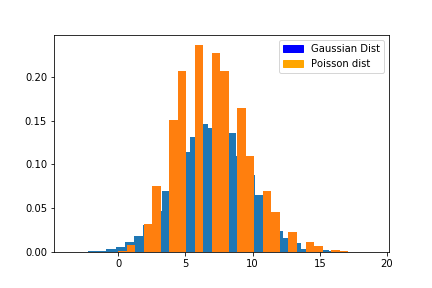
\includegraphics[width=10cm]{GVsP.png}
            \centering
            \caption{Plot of a gaussian distribution vs a poisson distribution}
        \end{figure}


        \item Do the same for two binomial distributions each at a time: one with p = 0.5 and 14 trials and another one with p = 0.005 and 1400 trials. What are the discrepancies between the two on-top-of-each- other plotted distributions? Which one of the binomial distributions is approximated better by the Gaussian distribution?
    \begin{figure}[h] 
        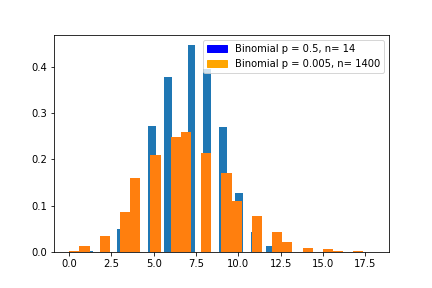
\includegraphics[width=10cm]{BVsB.png}
        \centering 
        \caption{Plot of 2 binomial distributions with different properties}
    \end{figure}
    \\
    Discrepancies between the Gaussian and the Poisson distribution are that the gaussian distribution is continuous which is seen by the fact that there are no gaps between the bins in the histogram. The Poisson and Binomial distribution are discrete and bounded at 0 hence the histogram stopping at 0 for them but not for the Gaussian. The Gaussian is also symmetric whereas the Poisson is not.
    \\
    The binomial distribution with p = 0.005 and n=1400 (orange) is better approximated by the gaussian distirbution as the histogram is more bell curved with an equal spread. This is due to having a higher n number and the probability being lower. Having more trials increases its approximation by a gaussian curve.


        \item Poisson Distrbution vs Binomial Distribution 
        \\
        As we can see the second binomial distribution with p = 0.005 and n = 1400 resembles the poisson distribution more.
        \begin{figure}
            \centering
            \begin{minipage}{.5\textwidth}
              \centering
              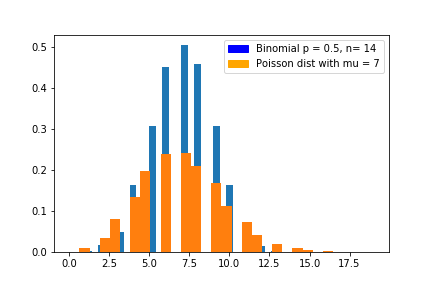
\includegraphics[width=1\linewidth]{B1vsP.png}
              \captionof{figure}{Plot of a binomial dist with p=0.5, n =14 vs a poisson dist with mu = 7}
              \label{fig:test1}
            \end{minipage}%
            \begin{minipage}{.5\textwidth}
              \centering
              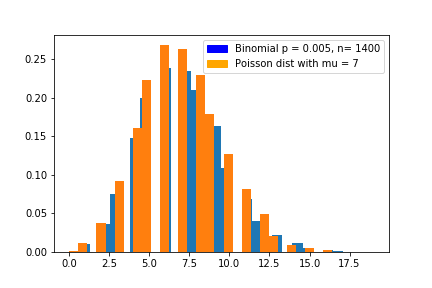
\includegraphics[width=1\linewidth]{B2vsP.png}
              \captionof{figure}{Plot of a binomial dist with p=0.005, n =1400 vs a poisson dist with mu = 7}
              \label{fig:test2}
            \end{minipage}
            \end{figure}
           
    \end{enumerate}

\end{enumerate}
\pagebreak


\item Appendix
\\
\begin{enumerate}
\item 2b(i) 
\\
\footnotesize{
\begin{lstlisting}[language=Python]
import matplotlib.pyplot as plt
import numpy as np
        
N = 10000
mu = 7
sigma = np.sqrt(mu)
        
G = np.random.normal(mu, sigma, N)
P = np.random.poisson(mu, N)
        
count, bins, ignored = plt.hist(G, 30, density=True)
        
count, bins, ignored = plt.hist(P, 30, density=True)
blue_patch = mpatches.Patch(color='blue', label='Gaussian Dist')
orange_patch = mpatches.Patch(color='orange', label='Poisson dist')
plt.legend(handles=[blue_patch, orange_patch])
plt.savefig('GVsP.png')
plt.show()
        
\end{lstlisting}
\item 2b(ii)
\begin{lstlisting}[language=Python]
import matplotlib.pyplot as plt
import numpy as np
import matplotlib.patches as mpatches


n_1 = 14 #number of trials
p_1 = 0.5 #probability 

n_2 = 1400 #number of trials
p_2 = 0.005 #probability


B_1 = np.random.binomial(n_1, p_1, N)
B_2 = np.random.binomial(n_2, p_2, N)
count, bins, ignored = plt.hist(B_1, 30, density=True)

count, bins, ignored = plt.hist(B_2, 30, density=True)
blue_patch = mpatches.Patch(color='blue', label='Binomial p = 0.5, n= 14')
orange_patch = mpatches.Patch(color='orange', label='Binomial p = 0.005, n= 1400')
plt.legend(handles=[blue_patch, orange_patch])
plt.savefig('BVsB.png')
plt.show()
\end{lstlisting}
\item Binomial Dist vs Gaussian Dists 
\\
\begin{lstlisting}[language=Python]
import matplotlib.pyplot as plt
import numpy as np
import matplotlib.patches as mpatches


n_1 = 14 #number of trials
p_1 = 0.5 #probability 

N = 10000
mu = 7
sigma = np.sqrt(mu)

B_1 = np.random.binomial(n_1, p_1, N)
P = np.random.poisson(mu, N)

count, bins, ignored = plt.hist(B_1, 30, density=True)
count, bins, ignored = plt.hist(P, 30, density=True)
blue_patch = mpatches.Patch(color='blue', label='Binomial p = 0.5, n= 14')
orange_patch = mpatches.Patch(color='orange', label='Poisson dist with mu = 7')
plt.legend(handles=[blue_patch, orange_patch])
plt.savefig('B1vsP.png')
plt.show()
\end{lstlisting}

\begin{lstlisting}[language=Python]
import matplotlib.pyplot as plt
import numpy as np
import matplotlib.patches as mpatches
    
    
n_2 = 1400 #number of trials
p_2 = 0.005 #probability
    
N = 10000
mu = 7
sigma = np.sqrt(mu)
    
B_2 = np.random.binomial(n_2, p_2, N)
P = np.random.poisson(mu, N)
    
count, bins, ignored = plt.hist(B_2, 30, density=True)
count, bins, ignored = plt.hist(P, 30, density=True)
blue_patch = mpatches.Patch(color='blue', label='Binomial p = 0.005, n= 1400')
orange_patch = mpatches.Patch(color='orange', label='Poisson dist with mu = 7')
plt.legend(handles=[blue_patch, orange_patch])
plt.savefig('B2vsP.png')
plt.show()

\end{lstlisting}
\item \underline{Python Code for Question 1}
\begin{lstlisting}[language=Python]
    import matplotlib.pyplot as plt
    import numpy as np
    from numpy.random import rand
    from numpy.random import seed
    import random
    from scipy.stats import pearsonr
    
    # seed random number generator
    seed(np.random.randint(1,100))
    
    n=10
    
    L = np.random.randint(1,10,n) #random integer between 1 and 10 for length
    W = np.random.randint(1,10,n) #randm integer between 1 and 10 for width
    #L = np.array([6,9,6,1,1,2,8,7,3,5])
    #W = np.array([6,3,5,3,5,8,8,2,8,1])
    H = np.full((1,n), 2.40) #height (and length and width) in m. array of 2.40s [1][10]
    carpet = L * W #area of carpet needed
    wallpaper = 2*(H*L) + 2*(H*W) #area of wallpaper needed
    
    #print(carpet)
    #print(wallpaper)
    #assuming uncertainties to be equal
    sigmaL = 0.01 #uncertainty in length
    sigmaW= 0.01 #uncertainty in width
    sigmaH=0.01 #uncertainty in height
    
    covLW = np.cov(L,W) #covariance between length and width
    covHL = np.cov(H,L) #covariance between height and lenght
    covHW = np.cov(H,W) #covariance between ehight and width
    
    sigmaCarpet = carpet * np.sqrt((sigmaL/L)**2 + (sigmaW/W)**2 + (2*(abs(covLW[0][1]/(L*W))))) #uncertainty in amount of carpet needed
    sigmaHL = (H*L) * np.sqrt((sigmaH/H)**2 + (sigmaL/L)**2 + (2*(abs(covHL[0][1]/(H*L))))) #uncertainty in H*L C in notes
    sigmaHW = (H*W) * np.sqrt((sigmaH/H)**2 + (sigmaW/W)**2 + (2*(abs(covHW[0][1]/(H*W))))) #uncertainty in H*W D in notes
    
    covCD = np.cov(H*L, H*W) #covariance between C and D or the height length and height width
    
    sigmaWallpaper = np.sqrt((4 * sigmaHL**2) + (4* sigmaHW**2)+ (8*abs(covCD[0][1]))) #uncertainty in wallpaper
    
    print(len)
    
    print(len(sigmaHL))
    print(len(sigmaHW))
    
    print(len(sigmaWallpaper))
    print(len(sigmaCarpet))
    
    covCaWa= np.cov(sigmaCarpet, sigmaWallpaper)   #covariance between carpet and wallpaper uncertainties
    corr2,_ = pearsonr(sigmaCarpet,sigmaWallpaper)
    
    #np.std(L) #std dev for L
    #np.std(W) #std dev for W
    
    #calculating the covariance between the uncertainties in the carpet and wallpaper
    sigmaC_s = sigmaCarpet**2
    sigmaWa_s = sigmaWallpaper**2
    sumsigmaC = np.sum(sigmaCarpet)
    sumsigmaWa = np.sum(sigmaWallpaper)
    sumC2 = np.sum(sigmaC_s)
    sumWa2 = np.sum(sigmaWa_s)
    
    covCW = n*(np.sum(sigmaCarpet*sigmaWallpaper))-(np.sum(sigmaCarpet)*(np.sum(sigmaWallpaper)))
    
    rCW = covCW / (np.sqrt((n*sumC2 - sumsigmaC**2)*(n*sumWa2 - sumsigmaWa**2)))
    
    
    L_s = L**2
    W_s = W**2
    sumL = np.sum(L)
    sumW = np.sum(W)
    sumL2 = np.sum(L_s)
    sumW2 = np.sum(W_s)
    
    cov = n*(np.sum(L*W))-(np.sum(L)*(np.sum(W)))
    
    r = cov / (np.sqrt((n*sumL2 - sumL**2)*(n*sumW2 - sumW**2)))
    
    corr2,_ = pearsonr(L,W)
    
                             
    print(L)
    print(W)
    print(H)
\end{lstlisting}

    }
\end{enumerate}

\end{enumerate}


\end{document}

